%REPORT TEMPLATE
%AUTHOR: RUI QU  
%EMAIL: RQU@KTH.SE 

%----------------------------------------------------------------------------------------
%	PACKAGES AND DOCUMENT CONFIGURATIONS
%----------------------------------------------------------------------------------------

\documentclass{article}

%---Basic---
\usepackage{natbib} % Required to change bibliography style to APA
\usepackage{amsmath} % Required for some math elements 
\setlength\parindent{0pt} % Removes all indentation from paragraphs
\usepackage{listings}%Insert code
\usepackage{times} % Uncomment to use the Times New Roman font

%---Table---
\usepackage{multirow}%Table
\usepackage{booktabs}%Table Triple-lines
\usepackage{siunitx} % Provides the \SI{}{} and \si{} command for typesetting SI units

%---Figure---
\usepackage{graphicx} % Required for the inclusion of images
\usepackage{subfigure} % Required for multiple images
\usepackage{float} 

%---Pseudo-code in LaTeX---
\usepackage{minted} %Preference->engine->pdfTeX->Latex  ADD: -shell-escape
\usepackage{xcolor}
\definecolor{bg}{rgb}{0.95,0.95,0.95}

\usepackage{algorithm}
\usepackage{algpseudocode}
\usepackage{amsmath}
\renewcommand{\algorithmicrequire}{\textbf{Input:}}  % Use Input in the format of Algorithm
\renewcommand{\algorithmicensure}{\textbf{Output:}} % Use Output in the format of Algorithm

%---Appendix---
\usepackage{appendix}
\newcommand{\upcite}[1]{\textsuperscript{\textsuperscript{\cite{#1}}}} %Upcite

%----------------------------------------------------------------------------------------
%	DOCUMENT INFORMATION
%----------------------------------------------------------------------------------------

\begin{document}

\title{CS-E5710 Bayesian Data Analysis\\Assignment 5}                  
%\author{Rui Qu\\rui.qu@aalto.fi}
\maketitle

% If you wish to include an abstract, uncomment the lines below
% \begin{abstract}
% Abstract text
% \end{abstract}

%----------------------------------------------------------------------------------------
%	SECTION 1
%----------------------------------------------------------------------------------------

\textbf{NB} The complete source code is given in the appendix. $psry.py$ and $bioarraylp.py$ are given in GitHub BDA repository. \\

\textbf{Number of chains \&Warm-up length}\\

In this assignment, I generate 15 chains with the sample size of 2000 each, 30000 samples in total. I set the warm-up length to 500, it removes 7500 in total.

\begin{minted}[bgcolor=bg, linenos, fontsize=\footnotesize]{python} 
chains=generate_chains(sample_size=2000,number_of_chains=15,worm_up=500)
\end{minted}

\textbf{The function to generate starting point and its mechanism}\\

All the starting pos$[\alpha, \beta]$ is randomly selected within $[-2,4], [-5,30]$. Then sample the amount of sample size in each chain and remove worm-upnsize samples.
\begin{minted}[bgcolor=bg, linenos, fontsize=\footnotesize]{python} 
def generate_chains(sample_size, number_of_chains,worm_up):
    print('number of draws:', sample_size)
    chains = []
    for i in range(number_of_chains):
        pos = [random.randint(-2, 4), random.randint(-5, 30)]
        chain = [pos]
        for j in range(sample_size):
            next_pos= get_next_pos(chain[-1], cov_matrix)
            chain.append(next_pos)
        print('starting point:', i, pos, ' PSRF:', psrf(chain))
        chains.append(chain)
    wormup_chains = []
    for chain in chains:
        wormup_chains.append(chain[worm_up:])
    return wormup_chains
\end{minted}

Sample for each chain from the starting point by the function below. The prior is the same as Exercise 5 and given in the source code in Appendix. The log-likelihood is calculated by $bioassaylp.py$. Thus we could get the posterior. Finally we calculate the ratio and set:
\begin{equation}
r=\frac{p(\theta^*|y)}{p(\theta^{t-1}|y)}
\end{equation}
\begin{equation}
\theta^t=\begin{cases}\theta^*&\text{with probability min(r,1)}\\ \theta^{t-1}&\text{otherwise}\end{cases}
\end{equation}

\begin{minted}[bgcolor=bg, linenos, fontsize=\footnotesize]{python}  
def get_next_pos(pos, cov):

    sample_pos = stats.multivariate_normal.rvs(pos, cov, size=1)
    sample_pos = np.array(sample_pos)

    likelihood_sample_pos = bioassaylp(sample_pos[0], sample_pos[1],
    	doses,deaths,animals)
    likelihood_pos = bioassaylp(pos[0],pos[1],doses,deaths,animals)

    prior_multivar_nor = stats.multivariate_normal(mean, cov_matrix)
    prior_sample_pos = prior_multivar_nor.pdf(sample_pos)
    prior_pos = prior_multivar_nor.pdf(pos)

    post_sample_pos=np.exp(likelihood_sample_pos)*prior_sample_pos
    post_pos = np.exp(likelihood_pos) * prior_pos

    ratio = post_sample_pos / post_pos

    if ratio >= 1:
        return sample_pos
    else:
        uniform_random_sample = stats.uniform(0,1).rvs(1)[0]
        if uniform_random_sample < ratio:
            return sample_pos 

    return pos
\end{minted}

\textbf{Number of draws per chain: 2000}\\

starting point: $[\alpha,\beta]$, PSRF:$[\hat{R}_{\alpha},\hat{R}_{\beta}]$\\

starting point: 0 [-1, 22]  PSRF: [0.99953966 1.00115549]\\
starting point: 1 [-1, 18]  PSRF: [1.00300136 1.00043561]\\
starting point: 2 [4, -4]  PSRF: [1.00258921 1.00310262]\\
starting point: 3 [4, 24]  PSRF: [1.02379704 1.0067836 ]\\
starting point: 4 [4, 5]  PSRF: [1.03105289 1.00568887]\\
starting point: 5 [-1, -1]  PSRF: [1.00523091 1.00300979]\\
starting point: 6 [3, 7]  PSRF: [1.00014292 1.00070187]\\
starting point: 7 [0, 14]  PSRF: [1.01720803 1.00254551]\\
starting point: 8 [4, 22]  PSRF: [1.00356257 1.02245706]\\
starting point: 9 [-1, 6]  PSRF: [1.00041033 1.00351039]\\
starting point: 10 [1, 6]  PSRF: [1.01850026 1.01549591]\\
starting point: 11 [2, 21]  PSRF: [1.0004834  0.99977666]\\
starting point: 12 [3, 18]  PSRF: [1.00664012 1.01332502]\\
starting point: 13 [4, 2]  PSRF: [0.99955723 1.00034767]\\


\textbf{Proposal/jumping distribution}\\

It's calculated by multivariate normal distribution with the Gaussian prior in Exercise 4. The code is given below and merged into the two functions above.
\begin{minted}[bgcolor=bg, linenos, fontsize=\footnotesize]{python}  
    sample_pos = stats.multivariate_normal.rvs(pos, cov, size=1)
    sample_pos = np.array(sample_pos)
\end{minted}

\textbf{Rhat-values}\\
The Rhat-values(Potential Scale Reduction Factor) are calculated by function $psry$  in $psry.py$

The Rhat-values of my first test:

\begin{minted}[bgcolor=bg, linenos, fontsize=\footnotesize]{python} 
chains=generate_chains(sample_size=2000,number_of_chains=15,worm_up=500)
\end{minted}

starting point: $[\alpha,\beta]$, PSRF:$[\hat{R}_{\alpha},\hat{R}_{\beta}]$\\
 
starting point: 0 [-1, 22]  PSRF: [0.99953966 1.00115549]\\
starting point: 1 [-1, 18]  PSRF: [1.00300136 1.00043561]\\
starting point: 2 [4, -4]  PSRF: [1.00258921 1.00310262]\\
starting point: 3 [4, 24]  PSRF: [1.02379704 1.0067836 ]\\
starting point: 4 [4, 5]  PSRF: [1.03105289 1.00568887]\\
starting point: 5 [-1, -1]  PSRF: [1.00523091 1.00300979]\\
starting point: 6 [3, 7]  PSRF: [1.00014292 1.00070187]\\
starting point: 7 [0, 14]  PSRF: [1.01720803 1.00254551]\\
starting point: 8 [4, 22]  PSRF: [1.00356257 1.02245706]\\
starting point: 9 [-1, 6]  PSRF: [1.00041033 1.00351039]\\
starting point: 10 [1, 6]  PSRF: [1.01850026 1.01549591]\\
starting point: 11 [2, 21]  PSRF: [1.0004834  0.99977666]\\
starting point: 12 [3, 18]  PSRF: [1.00664012 1.01332502]\\
starting point: 13 [4, 2]  PSRF: [0.99955723 1.00034767]\\


The Rhat-values of my second test:
\begin{minted}[bgcolor=bg, linenos, fontsize=\footnotesize]{python} 
chains=generate_chains(sample_size=2000,number_of_chains=1,worm_up=500)
\end{minted}

starting point: 0 [3, 6]  PSRF: [1.00054878 1.00186486]\\


\textbf{Interpretation of Rhat-values}\\

The potential scale reduction factors is estimated by:
\begin{equation}
\hat{R}=\sqrt{\frac{\hat{var}+(\psi|y)}{W}}
\end{equation}
which declines to 1 as $n\rightarrow \infty$If the potential scale reduction is high, then we have reason to believe that proceeding with further simulations may improve our inference about the target distribution of the associated scalar estimand. If Rhat-value is not close to 1, it is believed that the testing samples may be not from the same distribution or may not converge. In my test all Rhat-values is around 1 which means the generated chains converge well.\\

\textbf{Plot the draw of $\alpha$ and $\beta$ (scatter plot)}\\

\begin{figure}[H]
\centering  
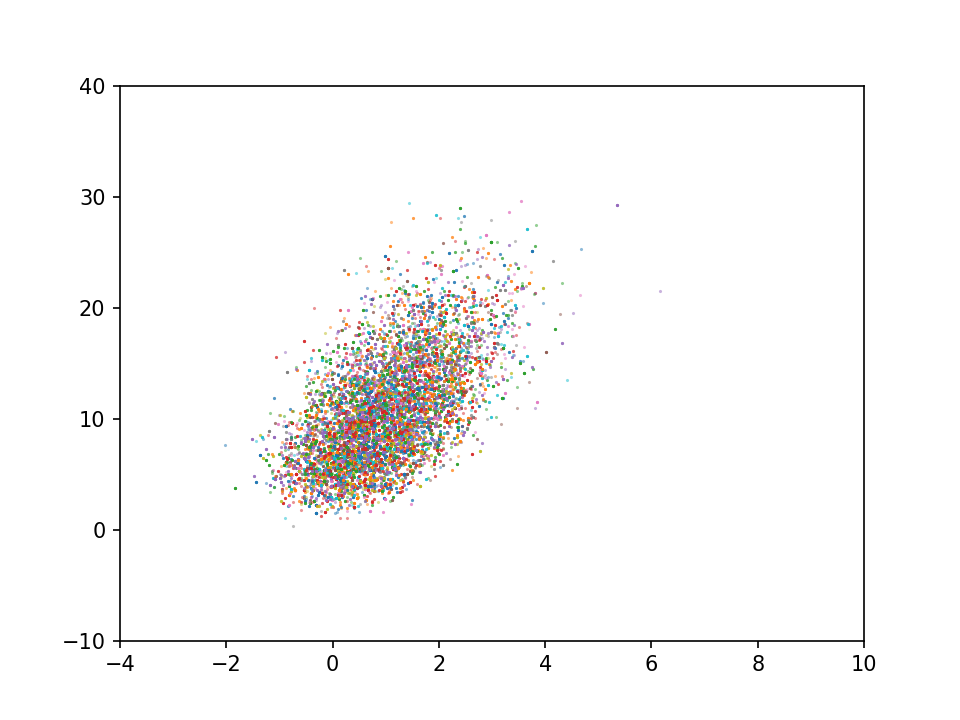
\includegraphics[scale=0.5]{1.png}
\caption{15 chains, 2000 samples/chain, warm-up length 500 }
\label{fig: label}
\end{figure}

\begin{figure}[H]
\centering  
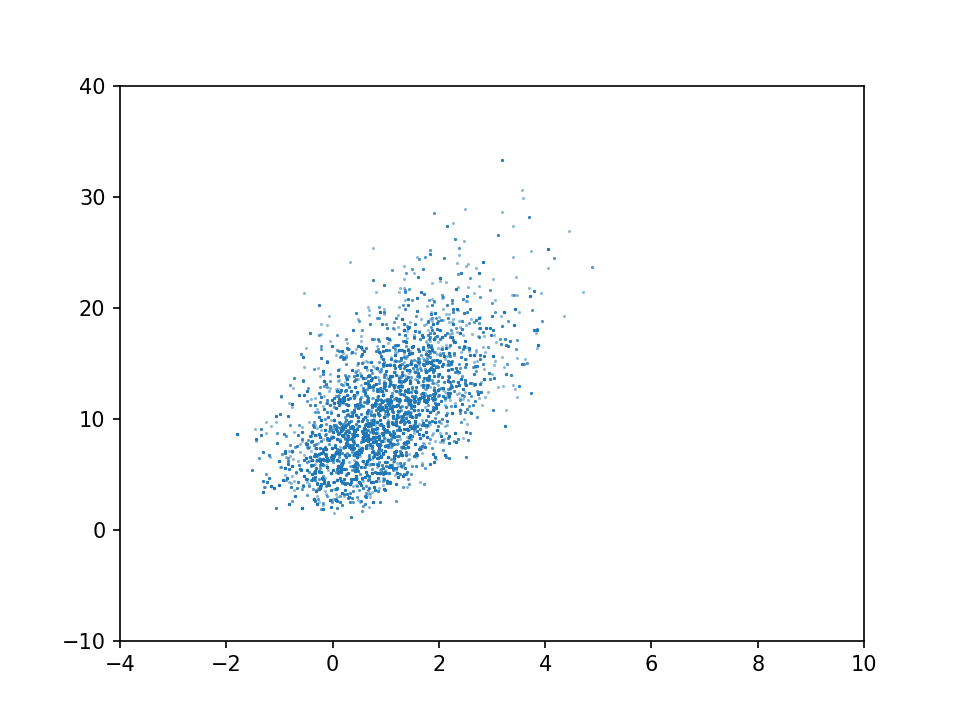
\includegraphics[scale=0.5]{2.png}
\caption{1 chains, 10000 samples/chain, warm-up length 500}
\label{fig: label}
\end{figure}

\clearpage
\appendix
\section{Code}

\begin{minted}[bgcolor=bg, linenos, fontsize=\footnotesize]{python} 

import matplotlib.pyplot as plt
from scipy import stats
import numpy as np
import random
from psrf import psrf
from bioarraylp import bioassaylp

sigma_a = 2
sigma_b = 10
mu_a = 0
mu_b = 10
corr = 0.5
cov_matrix = np.array([[sigma_a**2, corr * sigma_a * sigma_b], 
[corr * sigma_a * sigma_b, sigma_b**2]])
mean = np.array([mu_a, mu_b])

doses = np.array([-0.86, -0.3, -0.05, 0.72])
deaths = np.array([0, 1, 3, 5])
animals = np.array([5, 5, 5, 5])

def get_next_pos(pos, cov):

    sample_pos = stats.multivariate_normal.rvs(pos, cov, size=1)
    sample_pos = np.array(sample_pos)

    likelihood_sample_pos = bioassaylp(sample_pos[0], sample_pos[1],
    	doses,deaths,animals)
    likelihood_pos = bioassaylp(pos[0],pos[1],doses,deaths,animals)

    prior_multivar_nor = stats.multivariate_normal(mean, cov_matrix)
    prior_sample_pos = prior_multivar_nor.pdf(sample_pos)
    prior_pos = prior_multivar_nor.pdf(pos)

    post_sample_pos = np.exp(likelihood_sample_pos) * prior_sample_pos
    post_pos = np.exp(likelihood_pos) * prior_pos

    ratio = post_sample_pos / post_pos

    if ratio >= 1:
        return sample_pos
    else:
        uniform_random_sample = stats.uniform(0,1).rvs(1)[0]
        if uniform_random_sample < ratio:
            return sample_pos 

    return pos

def generate_chains(sample_size, number_of_chains,worm_up):
    print('number of draws:', sample_size)
    chains = []
    for i in range(number_of_chains):
        pos = [random.randint(-2, 4), random.randint(-5, 30)]
        chain = [pos]
        for j in range(sample_size):
            next_pos= get_next_pos(chain[-1], cov_matrix)
            chain.append(next_pos)
        print('starting point:', i, pos, ' PSRF:', psrf(chain))
        chains.append(chain)

    wormup_chains = []
    for chain in chains:
        wormup_chains.append(chain[worm_up:])
    return wormup_chains
    
chains=generate_chains(sample_size=2000,number_of_chains=15,worm_up=500)

for chain in chains:

    x = np.array(chain)[:, 0]
    y = np.array(chain)[:, 1]
    plt.xlim([-4, 10])
    plt.ylim([-10, 40])
    plt.plot(x,y,alpha=0.5,marker='.',linewidth=0,markersize=1)
  
plt.savefig('./1.png', dpi=150)
plt.show()

print('1 chain')
chain=generate_chains(sample_size=10000,number_of_chains=1,worm_up=500)[0]
print('Potential Scale Reduction Factor (PSRF)', psrf(chain))

x = np.array(chain)[:, 0]
y = np.array(chain)[:, 1]
plt.xlim([-4, 10])
plt.ylim([-10, 40])
plt.plot(x,y,alpha=0.5,marker='.',linewidth=0,markersize=1)
plt.savefig('./2', dpi=150)
plt.show()
\end{minted}





\end{document}